\section{Übung 2 – Diskrete Signale, Korrelation und Orthogonalität}

Dieses Aufgabenblatt behandelt zeitdiskrete Elementarsignale, ihre
Klassifikation als Energie- oder Leistungssignale sowie die Kreuz- und
Autokorrelation zeit\-diskreter und zeitkontinuierlicher Signale. Grundlage
sind die Abschnitte zu den elementaren diskreten Signalen
(\ref{sec:elementare-diskrete-signale}), zur Kreuzkorrelation
(\ref{sec:kreuzkorrelation}), zur Autokorrelation
(\ref{sec:autokorrelation}) und zu den Orthogonalsystemen
(\ref{sec:orthogonalsysteme}).

\begin{bemerkung}[Verwendete \texttt{rect}-Konvention]
Das Skript definiert den Rechteckimpuls asymmetrisch (Abschnitt~\ref{sec:elementare-analoge-signale}):
$$
\operatorname{rect}(u) = \begin{cases} 1 & , \quad 0 \leq u < 1 \\ 0 & , \quad \text{sonst.} \end{cases}
$$
Diese Konvention wird auf diesem Blatt durchgängig verwendet.
\end{bemerkung}

% ================================================================
\subsection*{Vorrechenaufgabe 2 – Zeitdiskrete Signale}
% ================================================================

Gegeben sind die Signale
$$
x_1[k] = \delta(k-1) + 2\,\delta(k-2) + \delta(k-3)
\qquad\text{und}\qquad
x_2[k] = \operatorname{rect}\!\left(\frac{k-2}{3}\right).
$$

% ---- a) --------------------------------------------------------
\subsubsection*{a) Skizze von $x_1[k]$ und $x_2[k]$}

\begin{beispiel}[Wertetabelle und Stem-Plot der Signale]

\textbf{Gegeben:} $x_1[k]=\delta(k-1)+2\delta(k-2)+\delta(k-3)$ und
$x_2[k]=\operatorname{rect}\!\big(\tfrac{k-2}{3}\big)$.

\textbf{Gesucht:} Darstellung beider Signale als Funktion des Index $k$.

\textbf{Formel} (diskrete Elementarsignale, Abschnitt~\ref{sec:elementare-diskrete-signale}):
Der Einheitsimpuls $\delta[k-k_0]$ ist genau bei $k=k_0$ gleich $1$; der
Rechteckimpuls $\operatorname{rect}\!\big(\tfrac{k-2}{3}\big)$ ist gleich $1$,
wenn $0 \leq \tfrac{k-2}{3} < 1$, also für $2 \leq k < 5$.

\textbf{Rechnung:}
$$
x_1[k]:\quad x_1[1]=1,\; x_1[2]=2,\; x_1[3]=1,\; \text{sonst }0.
$$
$$
x_2[k]:\quad x_2[2]=x_2[3]=x_2[4]=1,\; \text{sonst }0.
$$

\textbf{Lösung:}

\begin{center}
\begin{tikzpicture}
\begin{axis}[
  width=7.5cm, height=4.2cm, name=plot1,
  axis lines=middle, xlabel={$k$}, ylabel={$x_1[k]$},
  xmin=-1, xmax=5, ymin=0, ymax=2.4,
  xtick={0,1,2,3,4}, ytick={1,2},
  ycomb, mark=*, mark options={fill=accent}, color=accent, very thick,
]
\addplot coordinates {(1,1) (2,2) (3,1)};
\end{axis}
\begin{axis}[
  at={(plot1.right of east)}, xshift=1.2cm, anchor=west,
  width=7.5cm, height=4.2cm,
  axis lines=middle, xlabel={$k$}, ylabel={$x_2[k]$},
  xmin=-1, xmax=6, ymin=0, ymax=1.6,
  xtick={0,1,2,3,4,5}, ytick={1},
  ycomb, mark=*, mark options={fill=exercisegreen-fr}, color=exercisegreen-fr, very thick,
]
\addplot coordinates {(2,1) (3,1) (4,1)};
\end{axis}
\end{tikzpicture}
\end{center}

\end{beispiel}

% ---- b) --------------------------------------------------------
\subsubsection*{b) Kreuzkorrelationsfunktion $\varphi_{x_1 x_2}[\varkappa]$}

\begin{beispiel}[Diskrete Kreuzkorrelation zweier endlicher Folgen]

\textbf{Gegeben:} $x_1[k]$ und $x_2[k]$ aus Teil~a).

\textbf{Gesucht:} $\varphi_{x_1 x_2}[\varkappa]$ und ihr Verlauf.

\textbf{Formel} (Kreuzkorrelation reeller Energiesignale, Abschnitt~\ref{sec:kreuzkorrelation}):
$$
\varphi_{x_1 x_2}[\varkappa] = \sum_{k=-\infty}^{\infty} x_1[k]\,x_2[k+\varkappa]
$$

\textbf{Rechnung:}
Der Summand ist nur dort ungleich null, wo $x_1[k]\neq 0$ ($k\in\{1,2,3\}$)
\emph{und} $x_2[k+\varkappa]\neq 0$ ($2\leq k+\varkappa\leq 4$). Man wertet
$\varphi_{x_1 x_2}$ für jede relevante Verschiebung aus:
$$
\begin{aligned}
\varkappa=-1:&\quad x_1[3]\,x_2[2] = 1\cdot 1 = 1,\\
\varkappa=0:&\quad x_1[2]\,x_2[2] + x_1[3]\,x_2[3] = 2\cdot 1 + 1\cdot 1 = 3,\\
\varkappa=1:&\quad x_1[1]\,x_2[2] + x_1[2]\,x_2[3] + x_1[3]\,x_2[4] = 1 + 2 + 1 = 4,\\
\varkappa=2:&\quad x_1[1]\,x_2[3] + x_1[2]\,x_2[4] = 1 + 2 = 3,\\
\varkappa=3:&\quad x_1[1]\,x_2[4] = 1\cdot 1 = 1.
\end{aligned}
$$
Kontrolle: $\sum_\varkappa \varphi_{x_1 x_2}[\varkappa] = 1+3+4+3+1 = 12
= \big(\textstyle\sum_k x_1[k]\big)\big(\sum_k x_2[k]\big) = 4\cdot 3$. \checkmark

\textbf{Lösung:}
$$
\boxed{\;\varphi_{x_1 x_2}[\varkappa] = \{\,\underset{\varkappa=-1}{1},\;3,\;\underset{\varkappa=1}{4},\;3,\;1\,\},\qquad
\text{sonst }0.\;}
$$

\begin{center}
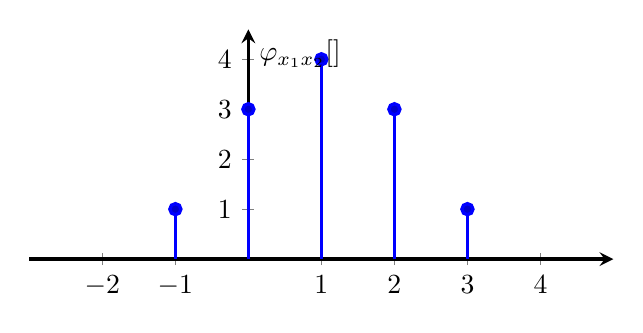
\begin{tikzpicture}
\begin{axis}[
  width=9cm, height=4.5cm,
  axis lines=middle, xlabel={$\varkappa$}, ylabel={$\varphi_{x_1 x_2}[\varkappa]$},
  xmin=-3, xmax=5, ymin=0, ymax=4.6,
  xtick={-2,-1,0,1,2,3,4}, ytick={1,2,3,4},
  ycomb, mark=*, mark options={fill=black}, very thick,
]
\addplot coordinates {(-1,1) (0,3) (1,4) (2,3) (3,1)};
\end{axis}
\end{tikzpicture}
\end{center}

Das Maximum liegt bei $\varkappa=1$: Um dieses Maß muss $x_2$ nach links
verschoben werden, damit sein Träger $\{2,3,4\}$ mit dem (gewichteten)
Schwerpunkt von $x_1$ zur Deckung kommt.

\end{beispiel}

% ================================================================
\subsection*{Aufgabe 2.1 – Zeitdiskrete Signale zeichnen}
% ================================================================

% ---- a) --------------------------------------------------------
\subsubsection*{a) $x[k] = 2 - 2\,\epsilon[k]$}

\begin{beispiel}[Konstante minus Sprungfunktion]

\textbf{Gegeben:} $x[k] = 2 - 2\,\epsilon[k]$ mit dem diskreten Einheitssprung
$\epsilon[k]$ ($\epsilon[k]=1$ für $k\geq 0$, sonst $0$).

\textbf{Gesucht:} Verlauf von $x[k]$.

\textbf{Formel} (Fallunterscheidung des Einheitssprungs, Abschnitt~\ref{sec:elementare-diskrete-signale}).

\textbf{Rechnung:}
$$
x[k] = \begin{cases} 2 - 0 = 2 & , \quad k < 0 \\ 2 - 2 = 0 & , \quad k \geq 0. \end{cases}
$$

\textbf{Lösung:}
\begin{center}
\begin{tikzpicture}
\begin{axis}[
  width=11cm, height=4cm, axis lines=middle, xlabel={$k$}, ylabel={$x[k]$},
  xmin=-5, xmax=5, ymin=0, ymax=2.4, xtick={-4,-3,-2,-1,0,1,2,3,4}, ytick={1,2},
  ycomb, mark=*, mark options={fill=accent}, color=accent, very thick,
]
\addplot coordinates {(-4,2) (-3,2) (-2,2) (-1,2)};
\addplot[only marks, mark=*, black] coordinates {(0,0) (1,0) (2,0) (3,0) (4,0)};
\end{axis}
\end{tikzpicture}
\end{center}
$x[k]$ ist eine „fallende`` Sprungfunktion: konstant $2$ für $k<0$ und $0$ für
$k\geq 0$.
\end{beispiel}

% ---- b) --------------------------------------------------------
\subsubsection*{b) $x[k] = \epsilon[k] - \epsilon[k-4] + \epsilon[k-8] - \epsilon[k-12]$}

\begin{beispiel}[Überlagerung verschobener Sprungfunktionen]

\textbf{Gegeben:} $x[k] = \epsilon[k] - \epsilon[k-4] + \epsilon[k-8] - \epsilon[k-12]$.

\textbf{Gesucht:} Verlauf von $x[k]$.

\textbf{Formel:} Jeder Term $\pm\epsilon[k-k_0]$ schaltet bei $k=k_0$ um $\pm 1$ um.

\textbf{Rechnung:}
$$
x[k] = \begin{cases}
0 & , \quad k < 0 \\
1 & , \quad 0 \leq k \leq 3 \\
1-1 = 0 & , \quad 4 \leq k \leq 7 \\
1-1+1 = 1 & , \quad 8 \leq k \leq 11 \\
1-1+1-1 = 0 & , \quad k \geq 12.
\end{cases}
$$

\textbf{Lösung:} Zwei Rechteckblöcke der Höhe $1$ auf $[0,3]$ und $[8,11]$.
\begin{center}
\begin{tikzpicture}
\begin{axis}[
  width=13cm, height=4cm, axis lines=middle, xlabel={$k$}, ylabel={$x[k]$},
  xmin=-2, xmax=14, ymin=0, ymax=1.5, xtick={0,2,4,6,8,10,12}, ytick={1},
  ycomb, mark=*, mark options={fill=accent}, color=accent, very thick,
]
\addplot coordinates {(0,1) (1,1) (2,1) (3,1) (8,1) (9,1) (10,1) (11,1)};
\end{axis}
\end{tikzpicture}
\end{center}
\end{beispiel}

% ---- c) --------------------------------------------------------
\subsubsection*{c) $x[k] = a^{-k}\,\epsilon[-k]$ mit $a=\tfrac12$}

\begin{beispiel}[Linksseitiges Exponentialsignal]

\textbf{Gegeben:} $x[k] = a^{-k}\,\epsilon[-k]$ mit $a=\tfrac12$.

\textbf{Gesucht:} Verlauf von $x[k]$.

\textbf{Rechnung:} Es ist $\epsilon[-k]=1$ für $k\leq 0$ und
$a^{-k} = \left(\tfrac12\right)^{-k} = 2^{k}$. Somit
$$
x[k] = \begin{cases} 2^{k} & , \quad k \leq 0 \\ 0 & , \quad k > 0. \end{cases}
\qquad
x[0]=1,\; x[-1]=\tfrac12,\; x[-2]=\tfrac14,\; \ldots
$$

\textbf{Lösung:} Das Signal ist linksseitig und klingt für $k\to -\infty$
geometrisch ab.
\begin{center}
\begin{tikzpicture}
\begin{axis}[
  width=11cm, height=4.2cm, axis lines=middle, xlabel={$k$}, ylabel={$x[k]$},
  xmin=-6, xmax=3, ymin=0, ymax=1.2, xtick={-5,-4,-3,-2,-1,0,1,2}, ytick={0.5,1},
  ycomb, mark=*, mark options={fill=accent}, color=accent, very thick,
]
\addplot coordinates {(-5,0.03125) (-4,0.0625) (-3,0.125) (-2,0.25) (-1,0.5) (0,1)};
\end{axis}
\end{tikzpicture}
\end{center}
\end{beispiel}

% ================================================================
\subsection*{Aufgabe 2.2 – Sprung und Einheitsimpuls}
% ================================================================

Aus den Bildern liest man die beiden Folgen ab:
$$
x_1[k] = (-1)^k \;\; \text{für } 0\leq k\leq 7,
\qquad
x_2[k] = \begin{cases} +1 & , \; 0\leq k\leq 4 \\ -1 & , \; 5\leq k\leq 9 \\ +1 & , \; 10\leq k\leq 14 \\ 0 & , \; \text{sonst.} \end{cases}
$$

% ---- x1 --------------------------------------------------------
\subsubsection*{$x_1[k]$ -- alternierende Folge}

\begin{beispiel}[Darstellung der alternierenden Folge]

\textbf{Gegeben:} $x_1[k]=1,-1,1,-1,1,-1,1,-1$ für $k=0,\ldots,7$.

\textbf{Gesucht:} Darstellung i) mit Einheitsimpulsen, ii) mit Sprungfunktionen.

\textbf{Formel:} $\delta[k-n]$ „setzt`` einen Einzelwert; $\epsilon[k-n]$ schaltet
eine Stufe.

\textbf{Rechnung / Lösung:}

\emph{i) Einheitsimpulse.}
$$
x_1[k] = \sum_{n=0}^{7} (-1)^n\,\delta[k-n]
= \delta[k] - \delta[k-1] + \delta[k-2] - \cdots - \delta[k-7].
$$

\emph{ii) Sprungfunktionen.} Jeder Vorzeichenwechsel entspricht einer Stufe der
Höhe $\pm 2$; die letzte Stufe $+1$ beendet die Folge:
$$
x_1[k] = \epsilon[k] + 2\sum_{n=1}^{7} (-1)^{n}\,\epsilon[k-n] + \epsilon[k-8].
$$
Kontrolle bei $k=7$: $1 - 2 + 2 - 2 + 2 - 2 + 2 - 2 = -1$; bei $k\geq 8$ addiert
der Term $+\epsilon[k-8]$ die $+1$, sodass $x_1[k]=0$. \checkmark

\begin{center}
\begin{tikzpicture}
\begin{axis}[
  width=12cm, height=4.5cm, axis lines=middle, xlabel={$k$}, ylabel={$x_1[k]$},
  xmin=-1, xmax=9, ymin=-1.4, ymax=1.4, xtick={0,1,2,3,4,5,6,7}, ytick={-1,1},
  ycomb, mark=*, mark options={fill=accent}, color=accent, very thick,
]
\addplot coordinates {(0,1) (1,-1) (2,1) (3,-1) (4,1) (5,-1) (6,1) (7,-1)};
\end{axis}
\end{tikzpicture}
\end{center}
\end{beispiel}

% ---- x2 --------------------------------------------------------
\subsubsection*{$x_2[k]$ -- Blockfolge}

\begin{beispiel}[Darstellung der Blockfolge]

\textbf{Gegeben:} $x_2[k]=+1$ auf $[0,4]$, $-1$ auf $[5,9]$, $+1$ auf $[10,14]$.

\textbf{Gesucht:} Darstellung i) mit Einheitsimpulsen, ii) mit Sprungfunktionen.

\textbf{Rechnung / Lösung:}

\emph{i) Einheitsimpulse.}
$$
x_2[k] = \sum_{n=0}^{4}\delta[k-n] \;-\; \sum_{n=5}^{9}\delta[k-n] \;+\; \sum_{n=10}^{14}\delta[k-n].
$$

\emph{ii) Sprungfunktionen.} Die Blockgrenzen liegen bei $k=0,5,10,15$:
$$
x_2[k] = \epsilon[k] - 2\,\epsilon[k-5] + 2\,\epsilon[k-10] - \epsilon[k-15].
$$
Kontrolle: $0\!\leq\! k\!\leq\!4\!:1$;\; $5\!\leq\! k\!\leq\!9\!:1-2=-1$;\;
$10\!\leq\! k\!\leq\!14\!:1-2+2=1$;\; $k\geq 15\!:1-2+2-1=0$. \checkmark

\begin{center}
\begin{tikzpicture}
\begin{axis}[
  width=14cm, height=4.5cm, axis lines=middle, xlabel={$k$}, ylabel={$x_2[k]$},
  xmin=-1, xmax=16, ymin=-1.4, ymax=1.4,
  xtick={0,2,4,6,8,10,12,14}, ytick={-1,1},
  ycomb, mark=*, mark options={fill=accent}, color=accent, very thick,
]
\addplot coordinates {(0,1) (1,1) (2,1) (3,1) (4,1) (5,-1) (6,-1) (7,-1) (8,-1) (9,-1) (10,1) (11,1) (12,1) (13,1) (14,1)};
\end{axis}
\end{tikzpicture}
\end{center}
\end{beispiel}

% ================================================================
\subsection*{Aufgabe 2.3 – Signaleigenschaften}
% ================================================================

Für zeitdiskrete Signale gelten (Abschnitt~\ref{sec:norm-energie-leistung} und~\ref{sec:leistung}):
$$
E = \sum_{k=-\infty}^{\infty} |x[k]|^2,
\qquad
P = \lim_{N\to\infty} \frac{1}{2N+1}\sum_{k=-N}^{N} |x[k]|^2.
$$
Ein \emph{Energiesignal} hat $0<E<\infty$ (und $P=0$), ein \emph{Leistungssignal}
$0<P<\infty$ (und $E\to\infty$). Der Bereichsmittelwert der nichtperiodischen
Signale wird über $k\in[-4,5]$ (also $10$ Werte) gebildet:
$\bar{x} = \tfrac{1}{10}\sum_{k=-4}^{5} x[k]$.

% ---- a) --------------------------------------------------------
\subsubsection*{a) $x[k] = e^{ak}\,\epsilon[k]$, $a\in\mathbb{R}$}

\begin{beispiel}[Kausales Exponentialsignal]

\textbf{Gegeben:} $x[k]=e^{ak}\epsilon[k]$.

\textbf{Gesucht:} Energie/Leistung, Klassifikation und Bereichsmittelwert.

\textbf{Formel} (geometrische Summe, vgl.\ Hinweis):
$\sum_{k=0}^{\infty} q^{k} = \tfrac{1}{1-q}$ für $|q|<1$.

\textbf{Rechnung:} Mit $|x[k]|^2 = e^{2ak}$ für $k\geq 0$:
$$
E = \sum_{k=0}^{\infty} e^{2ak} = \sum_{k=0}^{\infty}\big(e^{2a}\big)^{k}
= \frac{1}{1-e^{2a}} \quad\text{für } a<0.
$$
Für $a=0$ ist $x[k]=\epsilon[k]$ mit $P=\lim_{N\to\infty}\tfrac{N+1}{2N+1}=\tfrac12$;
für $a>0$ wächst $x[k]$ unbeschränkt ($E\to\infty$, $P\to\infty$).

Bereichsmittelwert ($a\neq 0$):
$$
\bar{x} = \frac{1}{10}\sum_{k=0}^{5} e^{ak}
= \frac{1}{10}\cdot\frac{1-e^{6a}}{1-e^{a}}, \qquad
\bar{x}\big|_{a=0} = \frac{6}{10}=0{,}6.
$$

\textbf{Lösung:}
$$
\boxed{\;a<0:\ \text{Energiesignal},\ E=\tfrac{1}{1-e^{2a}};\quad
a=0:\ \text{Leistungssignal},\ P=\tfrac12;\quad
a>0:\ \text{weder noch.}\;}
$$
\end{beispiel}

% ---- b) --------------------------------------------------------
\subsubsection*{b) $x_1[k]=\delta[k]$ und $x_2[k]=A\,\delta[k-2]$}

\begin{beispiel}[Einzelimpulse]

\textbf{Gegeben:} $x_1[k]=\delta[k]$, $x_2[k]=A\,\delta[k-2]$.

\textbf{Gesucht:} Energie/Leistung und Bereichsmittelwert.

\textbf{Rechnung:}
$$
E_{x_1} = \sum_k |\delta[k]|^2 = 1,\qquad
E_{x_2} = \sum_k |A\,\delta[k-2]|^2 = A^2.
$$
Beide besitzen endliche Energie, also $P=0$. Bereichsmittelwerte:
$$
\bar{x}_1 = \frac{1}{10}\cdot 1 = 0{,}1,\qquad
\bar{x}_2 = \frac{1}{10}\cdot A = \frac{A}{10}.
$$

\textbf{Lösung:}
$$
\boxed{\;\text{Beides Energiesignale: } E_{x_1}=1,\; E_{x_2}=A^2,\; P=0.\;}
$$
\end{beispiel}

% ---- c) --------------------------------------------------------
\subsubsection*{c) $x[k] = \epsilon[1-k]$}

\begin{beispiel}[Rückwärtsgerichtete Sprungfunktion]

\textbf{Gegeben:} $x[k]=\epsilon[1-k]$.

\textbf{Gesucht:} Energie/Leistung und Bereichsmittelwert.

\textbf{Rechnung:} $\epsilon[1-k]=1$ für $1-k\geq 0$, d.h.\ $k\leq 1$; sonst $0$.
Das Signal ist für unendlich viele $k$ ungleich null $\Rightarrow E\to\infty$.
$$
P = \lim_{N\to\infty}\frac{1}{2N+1}\underbrace{(N+2)}_{k=-N,\ldots,1}
= \frac{1}{2}.
$$
Bereichsmittelwert (nichtzahl $k\leq 1$ im Fenster: $k=-4,\ldots,1$, also $6$ Werte):
$$
\bar{x} = \frac{1}{10}\cdot 6 = 0{,}6.
$$

\textbf{Lösung:}
$$
\boxed{\;\text{Leistungssignal},\ P=\tfrac12,\ \bar{x}=0{,}6.\;}
$$
\end{beispiel}

% ---- d) --------------------------------------------------------
\subsubsection*{d) $x[k] = \operatorname{Im}\big\{\sqrt{2}\,e^{j\pi/4}\,e^{j\Omega k}\big\}$}

\begin{beispiel}[Reelles Sinussignal]

\textbf{Gegeben:} $\Omega = \tfrac{2\pi f}{f_A}$ mit $f=1\,\text{kHz}$, $f_A=8\,\text{kHz}$,
also $\Omega=\tfrac{\pi}{4}$.

\textbf{Gesucht:} Energie/Leistung, Klassifikation, Mittelwert.

\textbf{Rechnung:} Mit $\sqrt{2}\,e^{j\pi/4}=1+j$ folgt
$$
x[k] = \operatorname{Im}\big\{(1+j)\,e^{j\pi k/4}\big\}
= \sqrt{2}\,\sin\!\Big(\frac{\pi(k+1)}{4}\Big).
$$
Das Signal ist mit $N=8$ periodisch ($\Omega N = 2\pi$), also ein
Leistungssignal. Die Leistung eines Sinus der Amplitude $\hat{x}=\sqrt2$ ist
$P=\hat{x}^2/2 = 1$; der Mittelwert über eine Periode verschwindet.

\textbf{Lösung:}
$$
\boxed{\;\text{Leistungssignal},\ P=1,\ \bar{x}=0,\ \text{periodisch mit } N=8.\;}
$$
\end{beispiel}

% ---- e) --------------------------------------------------------
\subsubsection*{e) $\underline{x}[k] = \sqrt{2}\,e^{j\pi/4}\,e^{j\Omega k}$}

\begin{beispiel}[Komplexes Exponentialsignal]

\textbf{Gegeben:} $\Omega=\tfrac{2\pi f}{f_A}=\tfrac{\pi}{4}$ (wie d).

\textbf{Gesucht:} Energie/Leistung, Klassifikation, Mittelwert.

\textbf{Rechnung:} Der Betrag ist konstant:
$$
|\underline{x}[k]|^2 = \big|\sqrt{2}\,e^{j\pi/4}\big|^2\cdot\big|e^{j\Omega k}\big|^2 = 2.
$$
Damit $E\to\infty$ und
$$
P = \lim_{N\to\infty}\frac{1}{2N+1}\sum_{k=-N}^{N} 2 = 2.
$$
Über eine Periode ($N=8$) mittelt sich der rotierende Zeiger zu null:
$\bar{\underline{x}} = \sqrt2\,e^{j\pi/4}\cdot\tfrac1N\sum_{k=0}^{7} e^{j\pi k/4}=0$.

\textbf{Lösung:}
$$
\boxed{\;\text{Leistungssignal},\ P=2,\ \bar{\underline{x}}=0,\ \text{periodisch mit } N=8.\;}
$$
\end{beispiel}

% ================================================================
\subsection*{Aufgabe 2.4 – Auto- und Kreuzkorrelation}
% ================================================================

Für Energiesignale gilt (Abschnitte~\ref{sec:kreuzkorrelation},~\ref{sec:autokorrelation})
$\varphi_{xy}(\tau)=\int_{-\infty}^{\infty} x(t)\,y(t+\tau)\,\mathrm{d}t$.

% ---- a) --------------------------------------------------------
\subsubsection*{a) $x_1(t)=\operatorname{rect}(t/T)$, $x_2(t)=\operatorname{rect}(t/2T)$}

\begin{beispiel}[Korrelation zweier Rechtecke unterschiedlicher Breite]

\textbf{Gegeben:} $x_1(t)=1$ auf $[0,T)$, $x_2(t)=1$ auf $[0,2T)$.

\textbf{Gesucht:} $\varphi_{x_1 x_1}(\tau)$ und $\varphi_{x_1 x_2}(\tau)$.

\textbf{Rechnung:} Die AKF eines Rechtecks der Breite $T$ ist ein Dreieck; die KKF
(Breiten $T$ und $2T$) ein Trapez mit Plateau der Breite $T$:
$$
\varphi_{x_1 x_1}(\tau) = \int x_1(t)\,x_1(t+\tau)\,\mathrm{d}t = T-|\tau|,\quad |\tau|\leq T,
$$
$$
\varphi_{x_1 x_2}(\tau) = \begin{cases}
T+\tau & , \; -T\leq \tau \leq 0 \\
T & , \; 0\leq \tau \leq T \\
2T-\tau & , \; T\leq \tau \leq 2T \\
0 & , \; \text{sonst.}
\end{cases}
$$

\textbf{Lösung:}
$$
\boxed{\;\varphi_{x_1 x_1}(\tau)=T-|\tau|\ (|\tau|\leq T);\quad
\varphi_{x_1 x_2}(\tau)\ \text{Trapez, Plateau } T \text{ auf } [0,T].\;}
$$
\end{beispiel}

% ---- b) --------------------------------------------------------
\subsubsection*{b) $x_1(t)=\cos(2\pi t)$, $x_2(t)=\sin(2\pi t)$}

\begin{beispiel}[Korrelation periodischer Signale]

\textbf{Gegeben:} $x_1(t)=\cos(2\pi t)$, $x_2(t)=\sin(2\pi t)$; Periode $T_0=1$.

\textbf{Gesucht:} $\tilde{\varphi}_{x_1 x_1}(\tau)$ und $\tilde{\varphi}_{x_1 x_2}(\tau)$.

\textbf{Formel} (periodische Korrelation, Abschnitt~\ref{sec:kreuzkorrelation}):
$\tilde{\varphi}_{xy}(\tau)=\tfrac{1}{T_0}\int_0^{T_0} x(t)\,y(t+\tau)\,\mathrm{d}t$.

\textbf{Rechnung:} Mit den Additionstheoremen
$\cos a\cos b=\tfrac12[\cos(a-b)+\cos(a+b)]$ bzw.\
$\sin a\cos b=\tfrac12[\sin(a-b)+\sin(a+b)]$ und Wegmittelung der doppelten
Frequenz:
$$
\tilde{\varphi}_{x_1 x_1}(\tau) = \tfrac12\cos(2\pi\tau),\qquad
\tilde{\varphi}_{x_1 x_2}(\tau) = \tfrac12\sin(2\pi\tau).
$$

\textbf{Lösung:}
$$
\boxed{\;\tilde{\varphi}_{x_1 x_1}(\tau)=\tfrac12\cos(2\pi\tau),\quad
\tilde{\varphi}_{x_1 x_2}(\tau)=\tfrac12\sin(2\pi\tau).\;}
$$
Wegen $\tilde{\varphi}_{x_1 x_2}(0)=0$ sind $\cos$ und $\sin$ orthogonal.
\end{beispiel}

% ---- c) --------------------------------------------------------
\subsubsection*{c) $x_1(t)=\operatorname{rect}\!\big(\tfrac{t-T}{T}\big)$, $x_2(t)=\operatorname{rect}\!\big(\tfrac{t+T}{2T}\big)$}

\begin{beispiel}[Korrelation verschobener Rechtecke]

\textbf{Gegeben:} $x_1(t)=1$ auf $[T,2T)$, $x_2(t)=1$ auf $[-T,T)$.

\textbf{Gesucht:} $\varphi_{x_1 x_1}(\tau)$ und $\varphi_{x_1 x_2}(\tau)$.

\textbf{Rechnung:} Die AKF ist verschiebungsinvariant, also identisch zu a):
$\varphi_{x_1 x_1}(\tau)=T-|\tau|$ für $|\tau|\leq T$. Die KKF ergibt sich als
Überlappung von $[T,2T)$ mit dem um $\tau$ verschobenen Träger $[-T-\tau, T-\tau)$
von $x_2$:
$$
\varphi_{x_1 x_2}(\tau) = \begin{cases}
3T+\tau & , \; -3T\leq \tau \leq -2T \\
T & , \; -2T\leq \tau \leq -T \\
-\tau & , \; -T\leq \tau \leq 0 \\
0 & , \; \text{sonst.}
\end{cases}
$$

\textbf{Lösung:}
$$
\boxed{\;\varphi_{x_1 x_1}(\tau)=T-|\tau|\ (|\tau|\leq T);\quad
\varphi_{x_1 x_2}\ \text{Trapez, Plateau } T \text{ auf } [-2T,-T].\;}
$$
Das Maximum bei negativem $\tau$ spiegelt die Zeitverschiebung der beiden
Rechtecke gegeneinander wider.
\end{beispiel}

% ================================================================
\subsection*{Aufgabe 2.5 – Kreuzkorrelation}
% ================================================================

\begin{beispiel}[KKF eines Treppensignals mit einem Exponential-Rechteck]

\textbf{Gegeben:}
$$
z(t) = \begin{cases} A & , \; 2T\leq t < 4T \\ 2A & , \; 4T\leq t < 6T \\ 0 & , \; \text{sonst,} \end{cases}
\qquad
w(t) = A\,\operatorname{rect}\!\Big(\frac{t}{2T}\Big)\,e^{-t/T}
= A\,e^{-t/T}\ \text{auf } [0,2T).
$$

\textbf{Gesucht:} $\varphi_{wz}(\tau) = \int_{-\infty}^{\infty} w(t)\,z(t+\tau)\,\mathrm{d}t$.

\textbf{Formel} (KKF, Abschnitt~\ref{sec:kreuzkorrelation}) mit
$\int e^{-t/T}\,\mathrm{d}t = -T\,e^{-t/T}$.

\textbf{Rechnung:} $w(t)$ ist nur auf $[0,2T)$ ungleich null. Das um $\tau$ nach
links verschobene $z(t+\tau)$ besitzt die Sprungstellen bei $t=2T-\tau$,
$4T-\tau$, $6T-\tau$. Fallweise Integration liefert:

\emph{Fall $0\leq\tau\leq 2T$} (nur der $A$-Teil überlappt, von $2T-\tau$ bis $2T$):
$$
\varphi_{wz}(\tau) = A^2\!\!\int_{2T-\tau}^{2T}\! e^{-t/T}\,\mathrm{d}t
= A^2 T\,e^{-2}\big(e^{\tau/T}-1\big).
$$

\emph{Fall $2T\leq\tau\leq 4T$} ($A$-Teil auf $[0,4T-\tau)$, $2A$-Teil auf $[4T-\tau,2T)$):
$$
\varphi_{wz}(\tau) = A^2 T\Big(1 - 2e^{-2} + e^{(\tau-4T)/T}\Big).
$$

\emph{Fall $4T\leq\tau\leq 6T$} (nur der $2A$-Teil auf $[0,6T-\tau)$):
$$
\varphi_{wz}(\tau) = 2A^2 T\Big(1 - e^{(\tau-6T)/T}\Big).
$$
Nahtstellen-Kontrolle: bei $\tau=2T$ liefern beide oberen Fälle
$A^2T(1-e^{-2})$, bei $\tau=4T$ beide unteren $2A^2T(1-e^{-2})$; an $\tau=0$ und
$\tau=6T$ ist $\varphi_{wz}=0$. \checkmark

\textbf{Lösung:}
$$
\boxed{\;\varphi_{wz}(\tau)=\begin{cases}
0 & , \; \tau\leq 0 \\
A^2 T\,e^{-2}\big(e^{\tau/T}-1\big) & , \; 0\leq\tau\leq 2T \\
A^2 T\big(1-2e^{-2}+e^{(\tau-4T)/T}\big) & , \; 2T\leq\tau\leq 4T \\
2A^2 T\big(1-e^{(\tau-6T)/T}\big) & , \; 4T\leq\tau\leq 6T \\
0 & , \; \tau\geq 6T.
\end{cases}\;}
$$
Das Maximum $\varphi_{wz}(4T)=2A^2T(1-e^{-2})\approx 1{,}73\,A^2T$ tritt auf, wenn
der starke $2A$-Block von $z$ genau das (bei $t=0$ große) Fenster von $w$
überdeckt.
\end{beispiel}

% ================================================================
\subsection*{Aufgabe 2.6 – Energie und Korrelation}
% ================================================================

% ---- a) --------------------------------------------------------
\subsubsection*{a) KKF von Gaußimpuls und Deltafunktion}

\begin{beispiel}[Kreuzkorrelation mit einer verschobenen Deltafunktion]

\textbf{Gegeben:} $x_1(t)=e^{-\pi t^2}$, $x_2(t)=\delta(t-t_0)$.

\textbf{Gesucht:} $\varphi_{x_1 x_2}(\tau)$.

\textbf{Formel} (KKF und Ausblendeigenschaft der Deltafunktion, Abschnitt~\ref{sec:dirac-impuls}):
$$
\varphi_{x_1 x_2}(\tau) = \int_{-\infty}^{\infty} x_1(t)\,\delta(t+\tau-t_0)\,\mathrm{d}t.
$$

\textbf{Rechnung:} Die Deltafunktion blendet $t=t_0-\tau$ aus:
$$
\varphi_{x_1 x_2}(\tau) = e^{-\pi(t_0-\tau)^2} = e^{-\pi(\tau-t_0)^2}.
$$

\textbf{Lösung:}
$$
\boxed{\;\varphi_{x_1 x_2}(\tau) = e^{-\pi(\tau-t_0)^2}.\;}
$$
Die Korrelation mit einer Deltafunktion verschiebt den Gaußimpuls lediglich nach
$\tau=t_0$ (Abtast-/Verschiebeeigenschaft).
\end{beispiel}

% ---- b) --------------------------------------------------------
\subsubsection*{b) Energie und AKF des Gaußimpulses}

\begin{beispiel}[Energie und Autokorrelation des Gaußimpulses]

\textbf{Gegeben:} $x(t)=e^{-\pi t^2}$.

\textbf{Gesucht:} Energie $E$ und AKF $\varphi_{xx}(\tau)$.

\textbf{Formel} (Hinweis-Integral): $\int_0^{\infty} e^{-a^2 x^2}\,\mathrm{d}x=\tfrac{\sqrt{\pi}}{2a}$,
somit $\int_{-\infty}^{\infty} e^{-a^2 x^2}\,\mathrm{d}x=\tfrac{\sqrt{\pi}}{a}$.

\textbf{Rechnung:} Mit $a^2=2\pi$, d.h.\ $a=\sqrt{2\pi}$:
$$
E = \int_{-\infty}^{\infty} e^{-2\pi t^2}\,\mathrm{d}t
= \frac{\sqrt{\pi}}{\sqrt{2\pi}} = \frac{1}{\sqrt{2}}.
$$
Für die AKF wird der Exponent quadratisch ergänzt:
$$
-\pi t^2 - \pi(t+\tau)^2 = -2\pi\Big(t+\tfrac{\tau}{2}\Big)^2 - \tfrac{\pi}{2}\tau^2,
$$
$$
\varphi_{xx}(\tau) = e^{-\pi\tau^2/2}\!\int_{-\infty}^{\infty}\! e^{-2\pi(t+\tau/2)^2}\,\mathrm{d}t
= \frac{1}{\sqrt{2}}\,e^{-\pi\tau^2/2}.
$$

\textbf{Lösung:}
$$
\boxed{\;E = \frac{1}{\sqrt{2}}\approx 0{,}707,\qquad
\varphi_{xx}(\tau) = \frac{1}{\sqrt{2}}\,e^{-\pi\tau^2/2}.\;}
$$
Es gilt die Probe $\varphi_{xx}(0)=E$; die AKF eines Gaußimpulses ist wieder ein
(breiterer) Gaußimpuls.
\end{beispiel}

% ================================================================
\subsection*{Aufgabe 2.7 – Autokorrelation und Orthogonalität diskreter Signale}
% ================================================================

Aus den Bildern liest man (auf $k=0$ ausgerichtet) ab:
$$
\begin{aligned}
x_1[k] &= [\,1,1,1,1,1,1,1,1\,], & k&=0,\ldots,7, \\
x_2[k] &= [\,1,2,3,4,3,2,1\,], & k&=0,\ldots,6, \\
x_3[k] &= [\,1,1,1,1,-1,-1,-1,-1\,], & k&=0,\ldots,7, \\
x_4[k] &= [\,0{,}5,\,0{,}5,\,-0{,}5,\,-0{,}5,\,-0{,}5,\,-0{,}5,\,0{,}5,\,0{,}5\,], & k&=0,\ldots,7.
\end{aligned}
$$

% ---- AKFs ------------------------------------------------------
\subsubsection*{Autokorrelationsfunktionen}

\begin{beispiel}[AKF der vier Signale]

\textbf{Gegeben:} $x_1,\ldots,x_4$ wie oben.

\textbf{Gesucht:} $\varphi_{x_i x_i}[\varkappa]=\sum_k x_i[k]\,x_i[k+\varkappa]$ (Abschnitt~\ref{sec:autokorrelation}).

\textbf{Rechnung / Lösung:} (Die AKF ist gerade, es genügt $\varkappa\geq 0$.)

\emph{$x_1$ (Rechteck, $8$ Einsen):} Dreieck-AKF
$$
\varphi_{x_1 x_1}[\varkappa] = 8 - |\varkappa|,\quad |\varkappa|\leq 7.
$$

\emph{$x_2$ (Dreieck):}
$$
\varphi_{x_2 x_2}[\varkappa]\big|_{\varkappa=0,\ldots,6} = 44,\,40,\,31,\,20,\,10,\,4,\,1.
$$

\emph{$x_3$ (Sprung $+/-$):}
$$
\varphi_{x_3 x_3}[\varkappa]\big|_{\varkappa=0,\ldots,7} = 8,\,5,\,2,\,-1,\,-4,\,-3,\,-2,\,-1.
$$

\emph{$x_4$:}
$$
\varphi_{x_4 x_4}[\varkappa]\big|_{\varkappa=0,\ldots,7} = 2,\;0{,}75,\;-0{,}5,\;-0{,}75,\;-1,\;-0{,}25,\;0{,}5,\;0{,}25.
$$

\begin{center}
\begin{tikzpicture}
\begin{axis}[
  width=7.5cm, height=4cm, name=akf1,
  axis lines=middle, xlabel={$\varkappa$}, ylabel={$\varphi_{x_1 x_1}$},
  xmin=-8, xmax=8, ymin=0, ymax=9, xtick={-6,-4,-2,0,2,4,6}, ytick={4,8},
  ycomb, mark=*, mark size=1.2pt, mark options={fill=accent}, color=accent, thick,
]
\addplot coordinates {(-7,1)(-6,2)(-5,3)(-4,4)(-3,5)(-2,6)(-1,7)(0,8)(1,7)(2,6)(3,5)(4,4)(5,3)(6,2)(7,1)};
\end{axis}
\begin{axis}[
  at={(akf1.right of east)}, xshift=1.3cm, anchor=west,
  width=7.5cm, height=4cm,
  axis lines=middle, xlabel={$\varkappa$}, ylabel={$\varphi_{x_3 x_3}$},
  xmin=-8, xmax=8, ymin=-5, ymax=9, xtick={-6,-4,-2,0,2,4,6}, ytick={-4,4,8},
  ycomb, mark=*, mark size=1.2pt, mark options={fill=satzred-fr}, color=satzred-fr, thick,
]
\addplot coordinates {(-7,-1)(-6,-2)(-5,-3)(-4,-4)(-3,-1)(-2,2)(-1,5)(0,8)(1,5)(2,2)(3,-1)(4,-4)(5,-3)(6,-2)(7,-1)};
\end{axis}
\end{tikzpicture}
\end{center}

Alle AKF besitzen ihr Maximum bei $\varkappa=0$ (dort gleich der Signalenergie:
$8,\,44,\,8,\,2$).
\end{beispiel}

% ---- Orthogonalität --------------------------------------------
\subsubsection*{Orthogonalität}

\begin{beispiel}[Welche Signale sind orthogonal?]

\textbf{Gegeben:} $x_1,\ldots,x_4$.

\textbf{Gesucht:} Alle orthogonalen Paare.

\textbf{Formel} (Orthogonalität, Abschnitt~\ref{sec:orthogonalsysteme}):
$$
x_i \perp x_j \quad\Longleftrightarrow\quad
\varphi_{x_i x_j}[0] = \sum_k x_i[k]\,x_j[k] = 0.
$$

\textbf{Rechnung:} (Ausrichtung an $k=0$)
$$
\begin{aligned}
\langle x_1,x_3\rangle &= 4\cdot 1 + 4\cdot(-1) = 0, &
\langle x_1,x_4\rangle &= 2\cdot 0{,}5 + 4\cdot(-0{,}5) + 2\cdot 0{,}5 = 0, \\
\langle x_3,x_4\rangle &= 0{,}5+0{,}5-0{,}5-0{,}5+0{,}5+0{,}5-0{,}5-0{,}5 = 0, &
\langle x_1,x_2\rangle &= 1+2+3+4+3+2+1 = 16, \\
\langle x_2,x_3\rangle &= 1+2+3+4-3-2-1 = 4, &
\langle x_2,x_4\rangle &= -4.
\end{aligned}
$$

\textbf{Lösung:}
$$
\boxed{\;x_1\perp x_3,\quad x_1\perp x_4,\quad x_3\perp x_4
\;\Rightarrow\; \{x_1,x_3,x_4\}\ \text{sind paarweise orthogonal.}\;}
$$
$x_2$ ist zu keinem der anderen Signale orthogonal. Anschaulich hat $x_1$
(Gleichanteil) mit den vorzeichensymmetrischen Signalen $x_3$ und $x_4$ keinen
Überlapp, während der triangelförmige, rein positive Verlauf von $x_2$ stets
einen von null verschiedenen Beitrag liefert.
\end{beispiel}

% ================================================================
\subsection*{Aufgabe 2.8 – Log-Swept Chirp Signal}
% ================================================================

% ---- a) --------------------------------------------------------
\subsubsection*{a) Instantane Frequenz}

\begin{beispiel}[Herleitung der instantanen Frequenz]

\textbf{Gegeben:} Instantane Phase
$$
\varphi(t) = \frac{2\pi f_1 T}{\ln(f_2/f_1)}\left[\exp\!\Big(\frac{\ln(f_2/f_1)\,t}{T}\Big) - 1\right].
$$

\textbf{Gesucht:} Instantane (Kreis-)Frequenz $\omega(t)=\varphi'(t)$ bzw.\ $f(t)$.

\textbf{Rechnung:} Ableiten nach $t$ (innere Ableitung $\tfrac{\ln(f_2/f_1)}{T}$):
$$
\omega(t) = \varphi'(t)
= \frac{2\pi f_1 T}{\ln(f_2/f_1)}\cdot\frac{\ln(f_2/f_1)}{T}\,\exp\!\Big(\frac{\ln(f_2/f_1)\,t}{T}\Big)
= 2\pi f_1 \left(\frac{f_2}{f_1}\right)^{t/T}.
$$

\textbf{Lösung:}
$$
\boxed{\;f(t) = \frac{\omega(t)}{2\pi} = f_1\left(\frac{f_2}{f_1}\right)^{t/T}.\;}
$$
Es gilt $f(0)=f_1$ und $f(T)=f_2$; die Frequenz durchläuft den Bereich
$[f_1,f_2]$ \emph{exponentiell} (logarithmischer Sweep).
\end{beispiel}

% ---- b) --------------------------------------------------------
\subsubsection*{b) Erzeugung des Chirp-Signals}

\begin{beispiel}[Log-Sweep von 5\,Hz auf 15\,Hz]

\textbf{Gegeben / Gesucht:} Diskretes Chirp-Signal $x(t_k)=A\sin(\varphi(t_k))$
für $t_k = 0,\,\tfrac{1}{f_A},\,\ldots,\,T$; grafische Darstellung.

\textbf{Rechnung (Python):}
\begin{lstlisting}[style=python]
import numpy as np
import matplotlib.pyplot as plt

f1, f2, fA, T, A = 5.0, 15.0, 150.0, 2.0, 1.0
t = np.arange(0, T, 1.0/fA)          # diskrete Zeitachse t_k

# instantane Phase (log-swept chirp)
L = np.log(f2/f1)
phi = (2*np.pi*f1*T/L) * (np.exp(L*t/T) - 1.0)
x = A*np.sin(phi)

plt.figure(figsize=(9,3))
plt.plot(t, x)
plt.xlabel("t / s"); plt.ylabel("x(t)")
plt.title("Logarithmischer Frequenz-Sweep 5 Hz -> 15 Hz")
plt.tight_layout(); plt.show()
\end{lstlisting}

\textbf{Lösung:} Man erhält ein Sinussignal, dessen Schwingungen zum Ende hin
sichtbar dichter werden (die Momentanfrequenz steigt von $5$ auf $15$\,Hz an).
\end{beispiel}

% ---- c) --------------------------------------------------------
\subsubsection*{c) Audio-Chirp und Autokorrelation}

\begin{beispiel}[Audio-Chirp von 500\,Hz auf 2\,kHz]

\textbf{Gegeben / Gesucht:} Moduliertes Signal, seine Autokorrelation sowie
Speicherung als wav-Datei.

\textbf{Rechnung (Python):}
\begin{lstlisting}[style=python]
import numpy as np
import matplotlib.pyplot as plt
from scipy.io import wavfile

f1, f2, fA, T = 500.0, 2000.0, 8000.0, 2.0
t = np.arange(0, T, 1.0/fA)
L = np.log(f2/f1)
phi = (2*np.pi*f1*T/L) * (np.exp(L*t/T) - 1.0)
x = np.sin(phi)

# Autokorrelation (volle, symmetrische Faltung mit gespiegeltem Signal)
akf = np.correlate(x, x, mode="full")
lags = np.arange(-len(x)+1, len(x))

plt.plot(lags, akf); plt.xlabel("Verschiebung"); plt.ylabel("phi_xx")
plt.title("Autokorrelation des Log-Chirps"); plt.show()

# als 16-bit wav speichern
wavfile.write("chirp.wav", int(fA), (x*32767).astype(np.int16))
\end{lstlisting}

\textbf{Lösung:} Die Autokorrelation besitzt einen \emph{scharfen, schmalen Peak}
bei der Verschiebung $\varkappa=0$ und ist außerhalb nahezu null. Ein Chirp
ist damit -- trotz seiner zeitlichen Ausdehnung -- \emph{selbst\-un\-ähnlich} bei
Verschiebung; genau diese Eigenschaft nutzt man in der Messtechnik zur
Impulskompression (die AKF wirkt wie eine kurze Anregung mit hoher Energie). Beim
Anhören steigt der Ton hörbar von $500$\,Hz auf $2$\,kHz an.
\end{beispiel}

% ================================================================
\subsection*{Aufgabe 2.9 – Perfekte Sequenzen}
% ================================================================

\begin{beispiel}[Zyklische Korrelation einer perfekten Sequenz]

\textbf{Gegeben:} Die Folge (Länge $N=13$, $k=0,\ldots,12$)
$$
x[k] = [\,0,0,1,0,1,1,1,-1,-1,0,1,-1,1\,],
$$
sechsfach periodisch fortgesetzt.

\textbf{Gesucht:} Die von null verschiedenen Werte der (zyklischen)
Kreuz\-/Autokorrelation
$\varphi_{xx}(m)=\sum_{k=0}^{12} x[k]\,x[(k+m)_{\bmod 13}]$; Begriff „perfekte
Sequenz``.

\textbf{Rechnung (Python):}
\begin{lstlisting}[style=python]
import numpy as np
import matplotlib.pyplot as plt

x = np.array([0,0,1,0,1,1,1,-1,-1,0,1,-1,1])
N = len(x)                      # 13

phi = np.zeros(N)
for m in range(N):              # 'for'-Schleife ueber die Verschiebung
    s = 0
    for k in range(N):
        s += x[k]*x[(k+m) % N]  # zyklischer Index
    phi[m] = s

print(phi)                      # -> [9 0 0 0 0 0 0 0 0 0 0 0 0]
plt.stem(np.arange(N), phi)
plt.xlabel("m"); plt.ylabel("phi_xx(m)"); plt.show()
\end{lstlisting}

\textbf{Lösung:}
$$
\boxed{\;\varphi_{xx}(0) = \sum_k x[k]^2 = 9,\qquad \varphi_{xx}(m) = 0\ \text{für } m=1,\ldots,12.\;}
$$
Die zyklische Autokorrelation ist also ein reiner Diracstoß:
$\varphi_{xx}(m)=9\,\delta[m]$ (modulo $13$). Genau deshalb heißt die Folge
\emph{perfekte Sequenz} -- sie ist zu jeder von null verschiedenen zyklischen
Verschiebung ihrer selbst \emph{orthogonal}. Solche Sequenzen sind ideal für die
Kanalvermessung: Die Korrelation mit dem Empfangssignal liefert unmittelbar
einen sauberen Impuls (keine Nebenmaxima).
\end{beispiel}
